\chapter{Introduction}

\pagestyle{fancy}
\setcounter{page}{1}
\pagenumbering{arabic}

The exploration and production of oil and gas are essential activities for fulfilling the needs of the contemporary society. Delivering those resources is often associated with projects comprising high costs and risks, which can be reduced or mitigated by applying techniques of reservoir engineering and geosciences. Among those techniques is reservoir simulation, in which representative models are created to predict the behavior of fluid through porous or fractured media. Then, it is possible to forecast the reservoir behavior in different production scenarios and select the best development strategies.

%Some of their workflows include utilizing production and subsurface data for understanding reserves, calculating potential to production, and evaluating different production schemes.

According to \cite{Odeh1969}, for a hypothetical homogeneous and isotropic reservoir it is possible to utilize very simple models, the tank models, which defines the reservoir by its average proprieties (e.g., permeability, porosity, and pressure) in its whole. Those tank models are illustrated in Figure \ref{fig:8}, they are considered zero-dimensional since there is no variability of proprieties inside them. Considering a fairly homogeneous reservoir, it is possible to represent it by their average petrophysical values with a certain degree of accuracy. Thus, one could utilize Material Balance Equations (MBEs), the simplest form of mass conservation in a reservoir, for calculating initial hydrocarbon volumes in place and predicting production. On the other hand, this same approach is challenging when the reservoir presents relevant heterogeneities. \cite{Odeh1969} states that for reservoirs containing two different lithologies, but presenting petrophysical data homogeneously distributed inside each of them, it should be more accurate to represent it by two tank units, or grid blocks, connected one to another. Therefore, this model would be unidimensional with two grid blocks. In this case, there would be a flow between each of the units and the MBE should be utilized with the addition of an equation that models its flow (Darcy's law, if the medium is porous). This idea is the essence behind reservoir simulation and could be extended to different levels of heterogeneities. Reservoirs in that permeability are considerably different between both vertical and horizontal layers should be better represented by bidimensional or tridimensional models. Figures \ref{fig:8} to \ref{fig:10} shows examples of models with different dimensions. In a final analysis, the major advantage of modeling and simulation towards other reservoir engineering methods is their ability to account for those heterogeneities.
\nomenclature[A]{MBE}{Material Balance Equation}

According to \cite{Lie2015}, rock formations normally presents heterogeneities at all scales, from small pore channels to kilometer-wide reservoirs. Increasing resolution in reservoir models often enhances its accuracy. On the other hand, it also increases computational cost, making fine-grid models many times unpractical for field-wide history matching and simulation of development strategies. Therefore, there is a hierarchy of flow models for different scales of analysis. Some of those models include rock, core, facies, geological, and simulation. Figure \ref{fig:13} shows this hierarchy of models with their characteristic length unities. Since petrophysical data obtained by wireline logs and cores are in a small scale, many geological models present a high data resolution. It is often unpractical to assemble geological-model data to field-scale simulators and this data usually needs to be scaled up. Figure \ref{fig:11} shows the extreme heterogeneous data of the reservoir model for the SPE comparative project 10, a synthetic reservoir model built for performing comparative upscaling techniques and benchmarking. Figure \ref{fig:14} illustrates the scaling up of absolute permeabilities for a 128x128 grid to an 8x8 one. Upscaling, or homogenization, can be challenging in nonadditive proprieties such as permeability. According to \cite{Lie2015}, analytical solutions for nonadditive-propriety upscaling are only available for special cases, and most of the time the only form of homogenization is by fairly accurate approximations. Therefore, micro-scale effects are often non-represented by field-scale simulators.
\begin{figure}
	\centering
	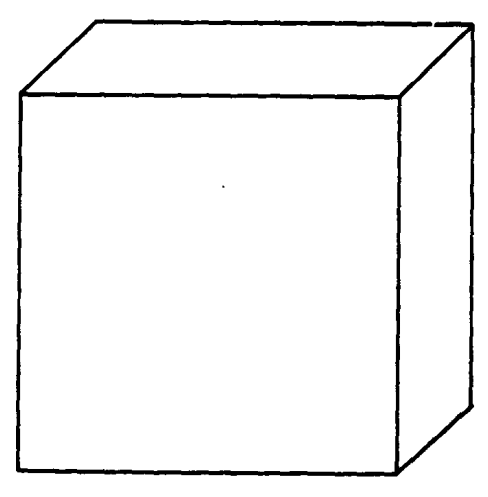
\includegraphics[width=0.2\linewidth]{Images/8}
	\caption{Representation of a tank model. Source: \cite{Odeh1969}.}
	\label{fig:8}
\end{figure}
\begin{figure}
	\centering
	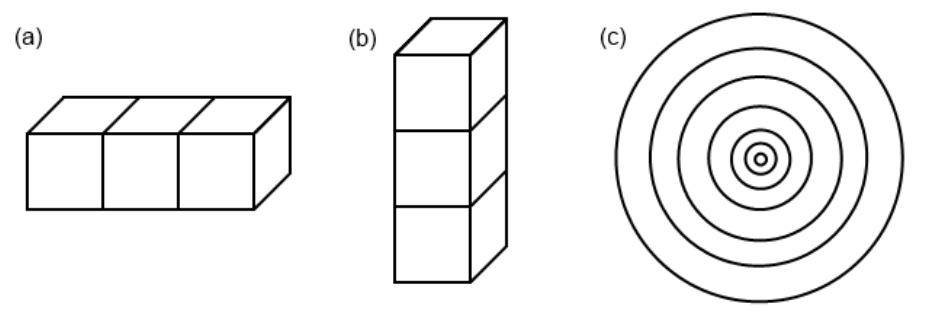
\includegraphics[width=0.6\linewidth]{Images/7}
	\caption{Representation of unidimensional models with different geometries. a) horizontal. b) vertical. c) radial. Source: \cite{Mattax1990}.}
	\label{fig:7}
\end{figure}
\begin{figure}
	\centering
	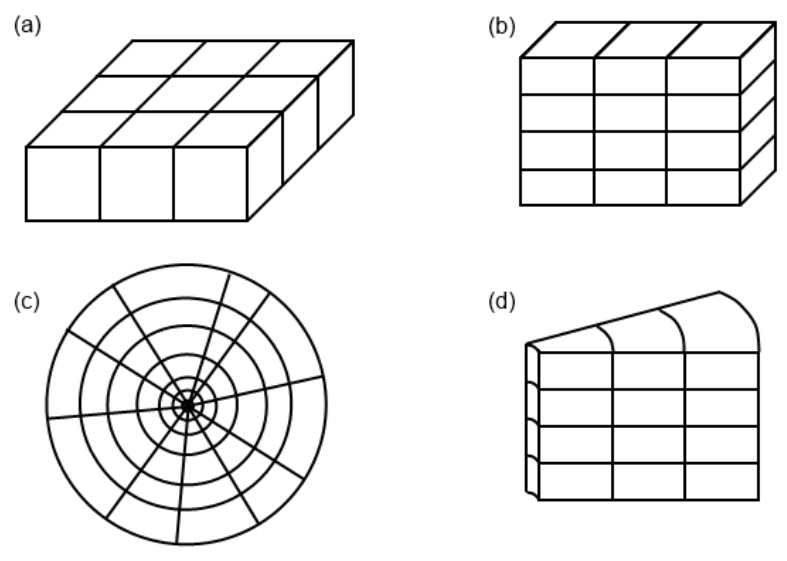
\includegraphics[width=0.5\linewidth]{Images/9}
	\caption{Representation of bi-dimensional models with different geometries. a) rectilinear horizontal. b) rectilinear vertical. c) radial horizontal. d) radial vertical. Source: \cite{Mattax1990}.}
	\label{fig:9}
\end{figure}
\begin{figure}
	\centering
	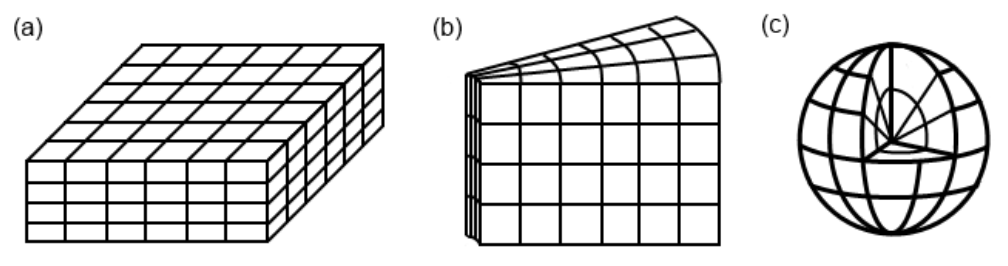
\includegraphics[width=0.7\linewidth]{Images/10}
	\caption{Representation of tridimensional models with different geometries. a) Cartesian. b) cylindrical. c) spheric.Source: \cite{Mattax1990}.}
	\label{fig:10}
\end{figure}
\begin{figure}
	\centering
	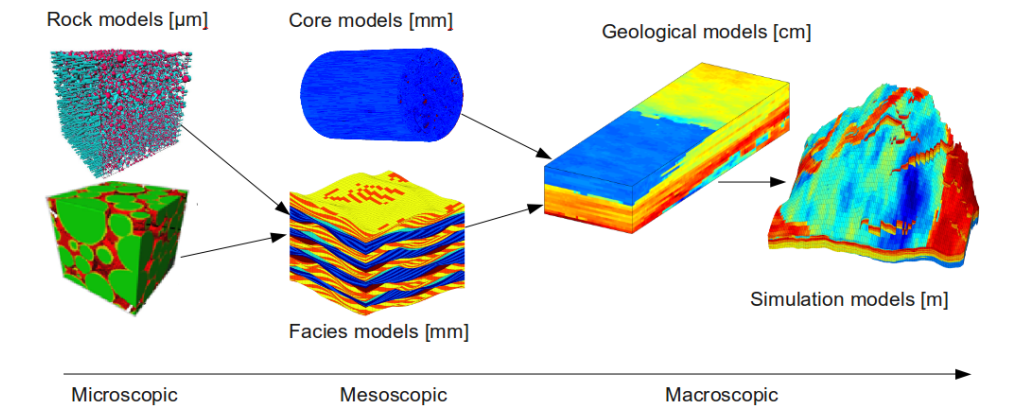
\includegraphics[width=0.9\linewidth]{Images/13}
	\caption{Representation of the hierarchy of flow models based in different levels of heterogeneity. Source: \cite{Lie2015}.}
	\label{fig:13}
\end{figure}
\begin{figure}
	\centering
	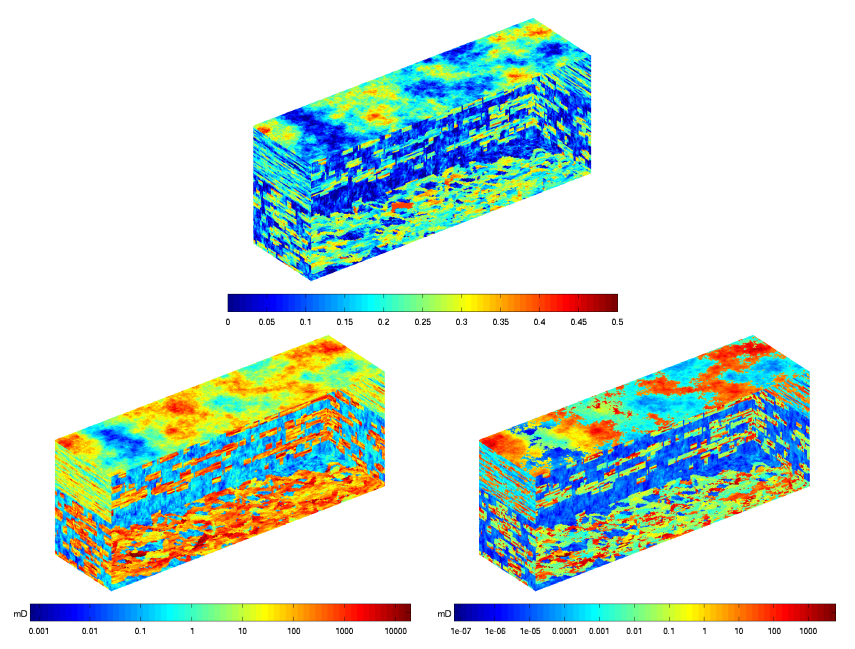
\includegraphics[width=0.7\linewidth]{Images/11}
	\caption{Reservoir rock properties for SPE 10 model. The upper image displays porosity, the lower left shows horizontal permeability, and the lower right the vertical permeability (in a logarithm color scale). Source: \cite{Lie2015}.}
	\label{fig:11}
\end{figure}
\begin{figure}
	\centering
	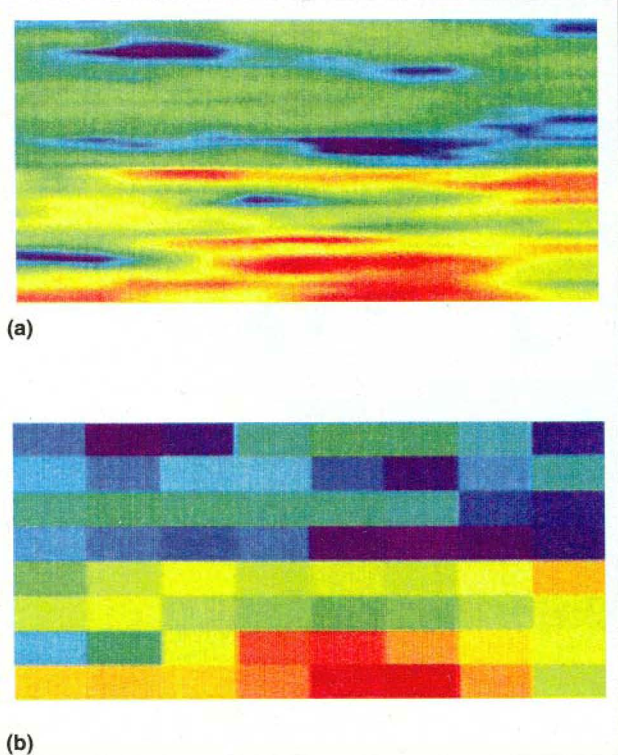
\includegraphics[width=0.4\linewidth]{Images/14}
	\caption{Absolute permeabilities. a) in 128x128 grid. b) in an 8x8 upscaled grid. Source: \cite{Christie1996}.}
	\label{fig:14}
\end{figure}
The operation of well testing normally consists of monitoring a pressure-transient response created by a change in flow rate. The obtained data is then compared with analytical solutions for inferring proprieties such as conductivity and storativity. Those evaluated proprieties represent some average of the scale of investigation, and small-scale heterogeneities might influence their results. This present project aims to study the heterogeneity loss in utilizing upscaled grids for synthetic well testing.
%According to \cite{paper_transient_upscaling}, the industry have been focused in upscaling methods based on steady-state, incompressible flow and few upscaling algorithms are robust enough for accounting other flow scenarios. While the traditional upscaling techniques could be acceptable for simulating conventional reservoirs with a short transient period, \cite{novel} many unconventional reservoirs nowadays present a pressure-transient with the length of decades or longer.
%This representation should account for errors, and traditional upscaling could present relevant inaccuracies. A quantitative evaluation of the appropriateness of averaging-based upscaling for transient or compressible flows is rare in the literature. This present project is expected to perform numerical analysis of the influence of grid size and average-based upscaling in compressible fluid, as well as in transient test.